% Chapter 1

\part{Satisfiability Problem: Definition and Relevance} % Main chapter title

\label{Chapter1} % For referencing the chapter elsewhere, use \ref{Chapter1} 

% ----------------------------------------------------------------------------------------

% Define some commands to keep the formatting separated from the content 
\newcommand{\keyword}[1]{\textbf{#1}}
\newcommand{\tabhead}[1]{\textbf{#1}}
\newcommand{\code}[1]{\texttt{#1}}
\newcommand{\file}[1]{\texttt{\bfseries#1}}
\newcommand{\option}[1]{\texttt{\itshape#1}}

% ----------------------------------------------------------------------------------------

\chapter{Logic}
\begin{itemize}
\item[TODO:]$\qquad$ Incluir introducción del problema.

\item[INFO:]
  \begin{itemize}
  \item Explicar que vamos a explicar en este capítulo.
  \item Handbook incluye una introducción histórica.
  \item Libro verde incluye una introducción intuitiva excelente.
\end{itemize}
\end{itemize}


In this chapter we present the bases of Logic and formal languages. Logic will provide us with a framework on which we will be able to define the Satisfiability Problem. We will present the area with formality, explaining only the things that will be necessary for our goal.


\section{Boolean Algebra}

The same way I started my journey on the university, we could have started this text right from the axioms, making a really romantic thesis. Nonetheless, given the goal we want to achieve, it seems excessive. We will refer to the commonly used \emph{Zermelo-Fraenkel axioms}, in order to have a point of reference, and therefore we will work without more considerations with sets and sets operations. We will put \emph{Zorn's lemma} to work, so the axiom of choice will also be needed, although in practice we will only work with finite sets of formulas.\\

Further on this section we will present Boolean Algebra in a classic lattice-based way that could be found in related literature. In particular we follow Introduction to mathematics of satisfiability\cite{marek2009introduction} for the definition of Booblean Algebra and Propositional Logic.

\begin{definition}
  A partial ordered set, also poset, is a pair $\{X, \le\}$ where $X$ is a set and $\le$ is a partial order of $X$. A chain $Y$ of $\{X, \le\}$ is a subset of $X$ where $\le$ is a total order. 
\end{definition}

\begin{proposition}[Zorn lemma]
  If every chain in a poset $\{X,\le\}$ is bounded, then $X$ possesses a maximal elements and for every $x\inX$ there is a maximal element $y$ such that $x\le y$.
\end{proposition}



\begin{definition} A lattice is a partial ordered set $\{X,\le\}$ where every pair of elements possesses a least upper bound and a greatest lower bound. A lattice has two new operations defined: given two elements $x,y\in X$
  \begin{itemize}
  \item $x\vee y$ denote the least upper bound.
  \item $x\wedge y$  denote the greatest lower bound.
  \end{itemize}
\end{definition}


  A lattice is complete if every subset has a unique largest element and a unique lowest element. A lattice is presented generally as a duple $\{L,\le\}$, a triple $\{X,\vee,\wedge\}$ and, whenever possible, is presented as a quintuple $\{X, \vee, \wedge, \top,\bot\}$ where $\top$ is the greatest element and $\bot$ the lowest element. A lattice is called distributive if $x\vee(y \wedge z) = (x\vee y) \wedge (x \vee z)$ and $x\wedge(y \vee z) = (x\wedge y) \vee (x \wedge z)$



With the concept of lattice just included, we present the \emph{Knaster and Tarski fixpoint theorem} fixpoint theorem. In order to do that we will introduce some notation. Given a function $f:\{L,\le\}\to \{L,\le\}$, a prefixpoint (resp. postfixpoint) is a point $x \in L$ such that $f(x) \le x$ (resp. $f(x) \ge x$). A fixpoint is a point that is both prefixpoint and postfixpoint. Note that, given that they exists, $\top$ and $bot$ are a prefixpoint and a postfixpoint of $f$ respectively.

\begin{theorem}[Knaster and Tarski fixpoint theorem \cite{marek2009introduction}]
  Let $f:\{L,\le\}\to \{L,\le\}$ be a monotone function in a complete lattice. Then:
  \begin{enumerate}
  \item $f$ has a least prefixpoint $l$ that is a fixpoint.
  \item $f$ has a largest postfixpoint $l$ that is a fixpoint.
  \end{enumerate}
\end{theorem}
\begin{proof}\\
  
  \begin{enumerate}
  \item We know that there is at least a prefixpoint. Let
    $$l = \bigwedge_{\{x\in X: x\text{ is a prefixpoint}\}} x $$. 
    Lets prove that $l$ is a fixpoint. Le $x$ be an arbitrary fixpoint, therefore, $l \le x \le f(x)$. Since $x$ was arbitrary, $f(l) \le l$. To show that it a fixpoint it suffices to see that $f(l)$ is a prefixpoint to, as $f$ is monotone.
  \item Apply the previous result on $f:\{L,\le\}\to \{L,\le\}$.
  \end{enumerate}
\end{proof}


\begin{definition}
  A \emph{Boolean algebra} is a distributive lattice  $\{X, \vee, \wedge, \top,\bot\}$ with an additional operation $\neg$, called complement or negation, such that for all $x\inX$:
  \begin{enumerate}
  \item $ x\wedge \neg x = \bot,\ x\vee \neg x = \top $
  \item $ \neg(x \vee y) = \neg x \wedge \neg y,  \neg(x \wedge y) = \neg x \vee \neg y$
  \item $\neg \neg x = x$
  \end{enumerate}
\end{definition}



\section{Propositional Logic}
Propositional logic is the framework that will allow us define the main topics of this text.  Let's define some concepts:
\begin{itemize}
\item An alphabet $A$ is an arbitrary non-empty set.
\item A symbol $a$ is an element of the alphabet.
\item A word $w = \{a_i:i\in 1,..,n\}$ is a finite sequence of symbols.
\item The collection of all possible words over an alphabet $A$ is denoted by $A^*$.
\item A language $L$ over $A$ is a subset of $A^*$.
\end{itemize}

For example, Spanish is a language with a well-known alphabet. Also, Spanish is a proper language over its alphabet as it is not empty, and it does not include all possible words.\\

When we talk about a logic system we are talking about a distinguished formal language. A formal language is defined by it syntax and its semantics. The syntax is the rules that define the language. They state what words over an alphabet are valid in the language. The semantics deal with the interpretations of the elements in the language. Usually this is achieved by assigning truth values to each word.\\

We will define now propositional logic, or zeroth-order-logic. \\

\begin{figure}[h]
  \begin{center}
    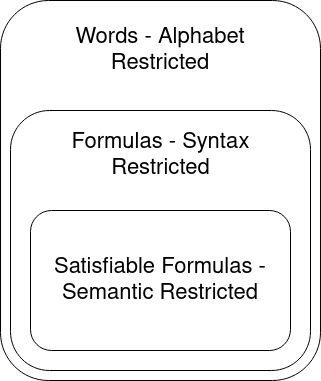
\includegraphics[width=5cm]{figures/sintax2.png}
    \caption{Diagram showing the different classes which are constructed on the formal language of Propositional Logic.}
  \end{center}
\end{figure} 

\subsection{Syntax of Propositional Logic}
We first start with the basic building blocks, which collectively form what is called the alphabet:
\begin{itemize}
\item Symbols $x,y,z$ for variables. As more variables are necessary sub-indexes will be used.
\item Unary operator $\neg$ (negation). A literal will refer to a variable or a negated variable.
  
\item Values 0 and 1. These values are often named as $\bot$ and $\top$ respectively.

\item Binary operators: $\wedge, \vee, \rightarrow, \oplus, \iff $
\end{itemize}


The words of Propositional Logic are called formulas.
\begin{definition}
  A Boolean formula is defined inductively:
  \begin{itemize}
  \item The constants 0 and 1 are formulas.
  \item Every variable is a formula.
  \item If $F$ is a formula, then $\neg  F$ is a formula.
  \item The concatenation with a binary operator of two formulas is a formula too.\\
  \end{itemize}
\end{definition}

Examples of formulas are $x\vee y$ or $x_1\wedge x_2 \vee  ( x_4 \vee \neg  x_3 \wedge (x_5\to x_6) \vee 0 )$.We should distinguish a special type of formula: the clauses. A clause  is a formula with the form $l_1\vee ... \vee l_n$ where $l_i, i \in 1,...,n$ are literals. Clauses are will be often regarded as a finite set of literals. Example of a clause is $(x_1\vee \neg x_4 \vee x_2)$. When regarded as a set every clause $C$ has a cardinal $|C|$, that represents the number of literals contained. \\

\subsection{Semantics of Propositional Logic}
When facing a way to provide semantic meaning to formulas the use of function In this section we will discuss to ways of providing meaning to the formulas: two-valued logic and three valued logic.\\ 

In two valued logic define the truth value of a formula by assigning a truth value(1 for Truth and 0 for False) to each variable. Note that we assign a meaning of truth to the constants 1 and 0, that until now where meaningless. The truth value of the formulas that involve operators are provide by their truth table.


\begin{table}[h]
  \begin{center}
    \begin{tabular}{|l|l|l|l|l|l|l|l|}
      \hline
      $p$ & $q$ & $\neg p$& $p\vee q$ & $p\wedge q$ & $p \oplus q$ & $p \to q $ & $p \iff q$  \\ 
      \hline
      0 & 0 & 1 & 0 & 0 & 0 & 1&1\\
      0 & 1 & 1 & 1 & 0 & 1 & 1&0\\
      1 & 0 & 0 & 1 & 0 & 1 & 0&0\\
      1 & 1 & 0 & 1 & 1 & 0 & 1&1\\\hline
    \end{tabular}
  \end{center}
  \caption{\label{tab:table-name}Truth tables of different operators in two valued logic.}
\end{table}


The truth value of a formula is therefore obtained by replacing each variable by their assigned constant and propagating the value. The tool that we will use to assign a truth value to each variable is the assignments
\begin{definition}
  An assignment is a function $\alpha$ from the $Form_{Var}$ to $Form_{Var}$, on which some variables $\{x_1,...,x_n \}$ are replaced by predefined constants $\{a_1,...,a_n\}$ respectively.\\
\end{definition}

An assignment that assigns a value to a variable $x$ is said to map the variable $x$. In two valued logic we will consider only assignment that maps all variables, and therefore all formulas are given a value by an assignment. We also see that any assignment generate a map from $Var$ to $\{0,1\}$. Conversely, any map from $Var$ to $\{0,1\}$ would uniquely represent a assignment $alpha$ over $Form_{Var}$. In practice when we talk about an assignment $\alpha$ we will refer indistinctly to either the function over $Form_{Var}$ or the mapping  over $Var$.\\

One can then \emph{apply} an assignment $\alpha$ to a formula $F$, denoting it by $F\alpha=\alpha(F)$. To describe an assignment we will use a set that pairs each variable to it value, i.e. $\alpha=\{x_1\to 1,...,x_n\to 0\}$. For example given an assignment $\alpha_0 = \{x_1 \to 1, x_2\to 1, x_3 \to 0, x_4 \to 1\}$ and $F_0=x_1\to (x_2\wedge x_4)$ then  $F_0\alpha_0=1 \to (1\wedge 1)= 1$. \\    

\begin{definition}
  An assignment is said to \emph{satisfy}  a formula $F$ if $F\alpha=1$ and in the case $F  \alpha = 0 $ it is said to \emph{falsify} the statement. A formula $F$ is called \emph{satisfiable} if is exists an assignment that satisfy it. Otherwise it is called \emph{unsatisfiable}.
\end{definition}


Note that we have a really restrictive constraint on assignments: they should map all variables.  This is so in order for an assignment to give a meaning to every formula. To ease this constraint we use three-valued logic. On three valued logic we have three significant: True or 1, False or 0, and unknown or $\upsilon$. Now the assignment will map every variable to one of these values. These new assignments will be called partial assignments, as they only map some variables to a truth value. We can propagate the previous values adding new rules.

\begin{table}[h]
  \begin{center}
    \begin{tabular}{|l|l|l|l|l|l|l|l|}
      \hline
      $p$ & $q$ & $\neg p$& $p\vee q$ & $p\wedge q$ & $p \oplus q$ & $p \to q $  & $p \iff q$  \\ 
      \hline
      
      \upsilon & 0 & \upsilon & \upsilon & 0 & \upsilon & \upsilon &\upsilon\\
      \upsilon & 1 & \upsilon & 1 & \upsilon & \upsilon & 1 &\upsilon\\
      0 & \upsilon & 1 & \upsilon & 0 & \upsilon & 1 &\upsilon\\
      1 & \upsilon & 0 & 1 & \upsilon & \upsilon & \upsilon &\upsilon\\
      \hline

    \end{tabular}
  \end{center}
  \caption{\label{tab:table-name}Truth table of different operators in three valued logic.}
\end{table}


In practice partial assignments will be only define by denoting only the variables that are mapped to either 0 or 1. We can see that the composition of assignments (seen as functions over $Form_{var}$ is also a partial assignment. Also, when applying a partial assignment to a formula, instead of mapping it to $\upsilon$ we will avoid operating over the variables assigned to $\upsilon$. For example given a partial assignment $\alpha_0 = \{x_1 \to 1, x_2\to 1, x_3 \to 0\}$ and $F_0=x_1\to (x_2\wedge x_4)$ then  $F_0\alpha_0=1 \to (1\wedge x_4)= 1 \to (x_4)$. Although $F_0$ is mapped to another formula by $\alpha_0$, $\alpha_0$ is still providing a meaning to it (the unknown meaning). \\



Partial assignments will be also used to iteratively \emph{expand} them: let $Var= \{x_i:i\in 1,...,n\}$ the set of variables and let $\alpha_1$ be partial assignment that map variables $[x_1\to a_1,...,x_j\to a_j]$ with $1<j<n$ and $a_j\in\{0,1\}$ for every $j$, we can expand it by choosing a nonempty subset  $A\subset\{a_k: k\in j+1,..,n\}$ and a value $c_x \in \{0,1\}$ for every $x\in A$. Then we can define:

$$
\alpha_2(x)=
\begin{cases}
  \alpha_1(x) & x \in \{x_i : i \in 1,...,n\},\\
  c_x & x\in A, \\
  \upsilon & \text{otherwise}.
\end{cases}
$$

We can see that $\alpha_2$ expands $\alpha_1$ in the sense that the truth value assigned to a formula by $\alpha_1$ holds in $\alpha_2$ if it where different that unknown. Therefore we are expanding the 'known' values of the formulas. Note that in the definition of $\alpha_1$ it where not necessary to state what variables were mapped to $\upsilon$ at it was implicit that every variable not listed were of unknown  value.\\

In practice we will try to avoid refer to this process whenever is evidently enough what is being done. Nonetheless partial assignments will be a central part of later explained algorithms such as DPLL[\ref{sec:dpll}]. When context is clear enough, assignments will be used for both assignments and partial assignments.\\

Arguably, the most special case of partial assignment are autarks assignments[\ref{sec:autark}]. An autark assignment is a partial assignment that simplify a formula in a sense latter explained.\\

Given an assignment or partial assignment $\alpha$ we will denote the set of variables mapped to either 0 or 1 by $Var(\alpha)$. Analogously, given a formula $F$, $Var(F)$ will denote the variables that appear in $F$. Note that if $F\in Form_{Var}$ then $Var(F)\in Var$ and it is not necessary that $Var(F)=Var$.\\


Two formulas $F,G$ are said to be equal, represented as $F\sim G$, if for every two-valued assignment $\alpha$ maps $F\alpha = G\alpha$. It follows from the equivalently properties on constants that $\sim$ is an equal relationship. This definition is really intuitive, as it define as equal the formulas that has the same meaning in every possible situation. \\



\label{def:linden}
With $\sim$ defined we can have what is called a \emph{Lindenbaum algebra}, as a quotient space of $Form = Form_{Var}$ by the relation $\sim$, denoted as $Form/\sim$. It follows that every operator respect the quotient space structure, i.e., for every $[\phi_1],[\phi_2]\in\ Form/\sim$:

\begin{itemize}
\item $\neg [\phi_1] = [\neg\phi_1]$
\item $ [\phi_1] \vee [\phi_2]= [\phi_1 \vee \phi_2]$
\item $ [\phi_1] \wedge [\phi_2]= [\phi_1 \wedge \phi_2]$
\end{itemize}

The interest of Lindenbaum algebra resides in the fact that $\{Form, \vee,\wedge,[1],[0]\}$ is a Boolean algebra, providing therefore a nexus between the algebraic formulation of the problem an its semantics.



\section{First order Logic}

\section{Modal Logic}


\chapter{Definition of the problem}
\section{Decision Problems}
Computability and complexity theory attempt to answer questions regarding how to efficiently solve real-world problems. In this section we provide a formal approach to the concept of problem, and its resolution.\\

We will study the complexity of functions. In order to standardize the approach we code the input of the function and the output of the functions using words over a finite alphabet. As for every finite alphabet $A$ there is a bijective mapping from $A^*$ to $\{0,1\}^*$ we can assume when its convenient that the alphabet is $\{0,1\}$. With this convention we are now ready to define what is a decision problem.

\begin{definition}[Decision Problem\cite{arora2009computational}]
  Given a language $L$ over an alphabet $A$, it has an associated decision problem that consist on, given a word $w\in A^*$ check whether $w$ is in $L$. 	
\end{definition}


When we have a named language, we refer indistinctly by this name to both the language and the associated decision problem. In order to define a decision problem is only needed to define a language over an alphabet. Therefore a decision problem may be defined implicitly, that is, as the set of the words in an alphabet that satisfy some condition. As semantics provide meaning to the languages, real world problems can be addressed as decision problems.

\section{Satisfiability Problem}
\subsection{Definition}

Given the previous definitions, we are now almost prepared to define the central part of this thesis: the satisfiability decision problem of propositional logic, SAT for short. To this end we define a special subset of formulas in Propositional Logic: the formulas in Conjunctive Normal Form.

\begin{definition}
  A formula $F$ is said to be in Conjunctive Normal Form ($CNF$) if $F$ is written as:
  $$F = C_1\wedge ... \wedge C_n$$
  Where $C_i$  are clauses.
\end{definition}

Note that every formula in $CNF$ can be regarded as a set of clauses. This approach is really useful in some contexts and will be often used.

\begin{definition}
  The Satisfiability Language of Propositional Logic (SAT) is the language over the alphabet of propositional logic that includes all formulas that are both satisfiable and in $CNF$.
\end{definition}

We will refer with the acronym $SAT$ to both the language and the associated decision problem. As checking if a formula is in CNF is a fairly simple syntax problem, we are only interested in asserting whether or not a formula in $CNF$ is satisfiable.

\begin{definition}
  A \emph{SAT-Solver} is an algorithm that, being given a formula $F$ in \emph{CNF} as input, answer whether or not is satisfiable.
\end{definition}

On chapter[\ref{chap:2}] we analyze the main SAT-solver developed in the literature. We will differentiate two types of SAT-Solver. The algorithms that, given enough time always output the correct result at the end are called \emph{complete}. The SAT-solvers that doesn't guaranty its result are called \emph{incomplete}. Of particular interest among incomplete SAT-solvers are the one-sided bounded error SAT-solvers. These are the called probabilistic algorithms, discussed on section\ref{sec:prob}   


\subsection{Variations}

The SAT decision problem quite a lot of variations, all of them of interest for certain complexity classes. We will list some of the most important, starting with two decision problems. The first of them is a natural generalization.

\begin{definition}
  The Generalized Satisfiability Language of Propositional Logic (GSAT) is the language over the alphabet of propositional logic that includes all formulas that are Satisfiable.
\end{definition}

With Tseitin's Theorem[\ref{the:Tseitin}] we can see that these two problems are in fact fairly similar. More often than not GSAT will be solved by solving an equivalent SAT problem. Analogously a \emph{GSAT-Solver}  is a SAT-solver that also accepts as inputs formulas not in CNF. Further on, every new problem will have a associated \emph{solver}, defined analogously.



\begin{definition}
  Let $F$ be a formula. $F$ is said to be $k$-CNF formula (equivalently a formula in $k$-CNF) if it is in CNF and $\forall C \in F, |C| = k$. $k$-SAT is the language of the formulas that are both satisfiable and in $k$-CNF.
\end{definition}

Other variations of SAT could be achieved by generalizing the concept of decision problem.

\begin{definition}[Function Problem]
  Let $A,B$ be two sets. Given a relation $R\subset A\times B$, it has an associated function problem that consists on, given a word $a\in X$ find a word $b\in B$ such that $(a,b)\in R$.
\end{definition}

\begin{definition}
  Let $CNF$ be the set of propositional formulas in CNF and $B$ the set of assignments.  The Satisfiability Function Problem of Propositional Logic (FSAT) is the function problem defined by the relation $$R=\{(F, b): F\in CNF, b \in B, Fb = 1\}.$$
\end{definition}
That is, is the problem of finding an assignment that satisfy a formula. Most of SAT-solvers not only try to solve SAT but also to solve FSAT, i.e., try to find an assignment that satisfy  the formula should it exists.
\begin{definition}
  Let $CNF$ be the set of propositional formulas in CNF and $B$ the set of assignments. The Maximum Satisfiability Problem (MAXSAT) is the problem. function problem defined by the relation $$R=\{(F,n) : F\in CNF, n = \max_{\alpha \in B}\{ | \{C\in F : C\alpha =1 \}| \}.$$
\end{definition}

That is, is the problem of finding the maximum number of assignments that can be satisfied simultaneously.\\

As we will see, most SAT-solvers are FSAT-solvers. In related literature the FSAT-solver are called constructive SAT-solvers, as they provide a constructive solution of the problem. Solvers that only solve sat are called non-constructive SAT-solvers. After presenting the concept of algorithmic complexity we will see that from a non constructive SAT-solver, a constructive SAT-solver can be made so that the latter is not much less efficient[\ref{sub:fromnon}].

\subsection{Constraint Satisfaction Problem}

We want to introduce the notion of Constraint Satisfaction Problem (CSP) because it defines a new optic over the SAT problem. CSP is, in fact, a generalization of SAT. On a CSP we want to find a solution among certain restriction. A example can of what is a CSP is watching film with your family. Each member impose its restrictions, and then we look for a film that satisfy them all. Should it happen that no film is found, we have a problem. This concept very naturally translates into propositional logic formulation, therefore giving propositional logic a greater area of work. Lets define CSP formally:

\begin{definition}[\cite{schoning2013satisfiability}]
  A \emph{Constraint Satisfaction Problem}(CSP) is a triple $\{X,D,C\}$ where:
  \begin{itemize}
  \item $X=\{x_1,...,x_n\}$ is the set of variables  occurring in the problem.
  \item $D=\{D_1,...,D_n\}$ is the set of the domains. Each $D_i={d_{i,1},..,d_{i,n_i}}$ is the domain of the variable $x_i$.
  \item $C=\{C_1,...,C_m\}$ is the set of constraints over the variables. For our intentions, these constraints must be written as:
    \begin{itemize}
    \item An equality, for example: $(x_i, x_j) = (d_{i,k}, d_{j,k'})$
    \item An inequality, for example: $(x_i, x_j) \ne (d_{i,k}, d_{ºj,k'})$
    \item Concatenation with a Propositional Logic operator of two equalities or inequalities, for example: $((x_1) = (d_{1,1}) \vee (x_2 \ne d_{2,5}) \wedge \neg((x_8,x_9) = (d_{8,3},d_{9,7}))$ .
    \end{itemize}
  \end{itemize}
\end{definition}
  The goal of a CSP is to found a mapping \[ \alpha:X\to \cup_{i\in 1,...,n} D_i\]
  
  such that every variable $x_i$ is mapped to a value on its associated domain $D_i$ and every constraint is satisfied. Such map will be called an \emph{assignment}, and if this map satisfy all constraints it is said that $\alpha$ \emph{satisfy} the CSP problem.\\


Note that we can use all our artillery from Propositional Logic as both an equalities and inequalities hold a binary truth value (True/False), therefore can be handled as Propositional Logic Variables. \\

The value in CSP resides on the simplicity of its formulations.  One can  easily define a CSP just by selecting the desired conditions of a solution and describing its context. Moreover, a lot of real world problems can be defined in terms of constraints. Constraint programming is a programming paradigm that consists on solving problems by defining them as CSP and letting CSP-solvers do the work.\\

SAT could be seen as a CSP where every domain is $\{0,1\}$ and each clause is a constraint. Therefore if we know how to solve CSP we know how to solve SAT. Let see the reverse.

\begin{proposition}
  Every CSP problem has an equivalent SAT problem.
\end{proposition}
\begin{proof}
  Let $ \{X,D,C\}$ be a CSP problem. To define a equivalent SAT problem we are going to define a SAT problem that can be solved if, and only if, the CSP problem can be solved. We will also request that from every assignment that satisfy the equivalent SAT problem, we can deduce an assignment that satisfy the CSP problem, and conversely. In order to define a SAT problem we are going to define a set of variable and a set of clauses to be satisfy.\\

  Our set of variables consists on a variable $y_{i,j}$ for each variable $x_i\in X$, and each value $d_{i,j}\in D_i$ that represent whether or not $x_i = d_{i,j}$. Now we define the set of clauses. The first to group of clauses are added for consistency reason, and the later is added in order to maintain the constraints.
  \begin{enumerate}
  \item $(y_{i,1}\vee ... \vee y_{i,n_i})$ for all $i\in 1,...,n$ that represents that every variable should take a value.
  \item $(\neg y_{i,j} \vee \neg y_{i,j})$ for all $i\in 1,...,n,\ j\in 1,...,n_i$ that represents that a variable can not take more that one value.
  \item $(y_{i,j})$ for every equality $x_i = d_{i,j}$ and $(\neg y_{i,j})$ for every inequality $x_i \ne d_{i,j}$. If two equalities or inequalities are expressed concatenated by a Propositional Logic operator we express the associated literals of the equalities and inequalities concatenated by the same Propositional Logic Operator. In order to express the resulting formulas as a CNF formula, we use Tseitin's Theorem. A proof of this theorem will be provided on [\ref{the:Tseitin}].
  \end{enumerate}

  If there is an assignment $\alpha$ that satisfy the associated SAT problem, then there is an assignment $\beta$ that satisfy the CSP problem such that $\beta(x_i=d_{i,j}$ if $\alpha(y_{i,j}) = 1$. From the clauses generated in 1. and 2. we can assert that such mapping is well defined, and from the clauses generated by 3. follow that $\beta$ satisfy all constraints.\\

  Conversely we can define an assignment $\alpha$ that satisfy the SAT problem from an assignment $\beta$ that satisfy the CSP problem by mapping $x_{i,j}$ 

$$
\alpha(x_{i})=
\begin{cases}
  1 & \beta(x{i}) = d_{i,j}\\
  0 & \text{otherwise}.
\end{cases}
$$

Therefore the CSP problem is solvable, if and only if, the SAT problem is satisfiable, and given a satisfying assignment of either the SAT or CSP problem we know how to generate a satisfying assignment of the other problem.
\end{proof}

In practice we will use CSP as a methodology of problem defining. It will provide easy solutions for complex problem, given that we solve SAT problem. More on this will be shown on [\ref{chap:3}]


\subsection{Autarks assignments}
\label{sec:autark}

Once we have defined what is a CNF formula and what is a problem we can proceed to define this anticipated concept.

\begin{definition}
  An partial assignment $\alpha$ is called autark for a CNF formula $F$ if for every clause $C \in F$ it happens that if $Var(C) \cap Var(\alpha) \ne \emptyset $ then $C\alpha = 1$.
\end{definition}

An autark assignment $alpha$  for a CNF formula $F$ is an assignment that satisfies all clauses that it 'touches'. These assignments provide simplifications of the CNF Formulas in the context of satisfiability, as they generate a new CNF formula $F\alpha$ that are satisfiable if, and only if,  $F$ is satisfiable. In set notation we can state that $\alpha$ is autark for $F$ if $F\alpha \subsetneq F$. Subsequently, trying to find simple autark assignment, i.e. assignment with not many variables,is a good praxis.\\


Should it happen that we have an algorithm for the Autarks Finding Problem, iterating it, we could find a satisfying assignment of any given formula if it exists such assignment, therefore solving FSAT.  Let's define the problem formally:

\begin{definition}
  Let $CNF$ the set of formulas in CNF and $Part$ the set of partial assignment. The Autark Finding Problem is the function problem defined by the relation:
  $$R = \{(F,\alpha): F \in CNF\wedge \forall C \in F( Var(C)\cap Var(\alpha)\ne\emptyset \implies C\alpha=1 )\}$$
\end{definition}

\begin{proposition} There is a reduction from FSAT to the Autark-Finding problem.
  \begin{proof} Suppose that an algorithm such that if it exists any autark it return one of them, and end with an error code otherwise is given.  \\

    Given a formula $F$, if there is not an autark then there is no solution for the SAT problem. If it finds an Autark-assignment $\alpha$ then we apply the same algorithm to $\alpha(F)$. Also, as it happens that $|Var(\alpha(F))|<|Var(F)|$ so we would only apply the algorithm finitely many times. Also, $F$ will be solvable if, and only if, $F\alpha$ is solvable.
  \end{proof}
  
\end{proposition}


\chapter{Complexity Classes and Relevance of the Problem}
\section{Models of Computation}
In this section we will discuss two computation models: Turing Machines and Circuits. We do not expect the text to be the first approximations to Turing machines, so we present a quick formal approach to the area. 

\subsection{Turing Machines}
Turing machines are arguably the epicenter of  models of computation. A Turing Machine  represents a long mechanical tape on which we are going to operate. The tape is divided in to discrete positions, such that we can see the tape as a one-dimensional array. Operating on this tape we can focus on a cell, scan its contents, overwrite  its contents or move to an adjacent cell. These operations try to resemble the process of human calculus, as done with paper and pencil when applying the long division method  for example. Formally:

\begin{definition}[Turing Machine \cite{hopcroft2007introduction}] We describe a Turing Machine as a 7-tuple $M=(Q, \Sigma, \Gamma, \delta, q_0, B, F)$ whose components have the following meanings:
  \begin{itemize}
  \item $Q$ the finite set of \emph{states} of the finite control.
  \item $\Sigma$ the finite set of \emph{input symbols}.
  \item $\Gamma$ the finite set of \emph{tape symbols}. $\Sigma$ is always a subset of $\Gamma$.
  \item  $\delta: Q\times \Gamma \to Q\times\Gamma\times\{L,R\}$ the transition function.
  \item $q_0$ the \emph{start state}.
  \item $B$ the \emph{blank symbol}.
  \item $F$ the \emph{accepting states}.
  \end{itemize}

  A configuration of a Turing machine is a triplet $C=(q,u,v)$ where $q\in Q$, $u,v\in \Gamma^*$. A configuration is accepting if $q\in F$.
\end{definition}

A configuration should be understand as a state of the machine, where $q$ is the current state, $u$ the part of the tape left to the cell on which we focus and $v$ is the part of the tape right to the cell we focus, starting on it.\\

As a brief note before going on, we have not define the empty word yet, as in propositional logic is not a valid formula so it lacks our interest until now. We will note the empty word as $\epsilon$ and would consist of an empty sequence of symbols. We can  now define a relation between configurations:

\begin{definition}
  Let $M$ be a Turing Machine and $C=(q,u,v)$, $C'=(q,u,v)$ be two configurations of $M$. We say that $C\vdash C'$ if there is a transition $\delta (q,v_1) = (q', b, D) $ with $D\in{L,R}$ and:
  \begin{itemize}
  \item if $D=L$, then if $u=u_1...u_n$ and $v = v_1...v_m$, it should happen that $u' = u_1...u_{n-1}$ and $v' = u_n bv_2...v_n$ with two exceptions:
    \begin{itemize}
    \item if $u=\epsilon$ then $u' = \epsilon$ and $v' = bv_2...v_n$
    \item if $v = v_1$ and $b =B$ then $u'=u_1...u_{n-1}$ and $v' = u_n$.
    \end{itemize}

  \item if $D=R$, then if $u=u_1...u_n$ and $v = v_1...v_m$, it should happen that $u' = u_1...u_{n}b$ and $v' = v_2...v_n$ with two exceptions:
    \begin{itemize}
    \item if $u=\epsilon$ then $u' = b$ and $v' =v_2...v_n$
    \item if $v = v_1$ and $b =B$ then $u'=u_1...u_{n-1}$ and $v' = \epsilon$.
    \end{itemize}
  \end{itemize}

  Note that on both cases the two exceptions can be given simultaneously (if $b = B$) and then give $(q, \epsilon, u_1) \vdash (q', \epsilon, B)$. We say $C\vdash^* C'$ if there exists a finite sequence $\{C_i\}_{i\in 1,...,n}$ such that $C_1 = C$, $C_n=C'$ and $C_i\vdash C_{i+1}$ for every $i\in 1,...,n-1$.  
  \end{definition}

  A Turing machine solves a decision problem, i.e. having an alphabet $\Sigma$  (its input alphabet) it takes a word in $\Sigma^*$ and decides whether it belongs to a language or not.The intuitive idea is that we write the word in question on the tape and the machine tells us the results after some computations. In this way we will consider that a word belongs to the language decided by the Turing machine if and only if it is \emph{accepted} by that machine. Let's define when this concept.

  \begin{definition}
     Let $M$ be a Turing Machine. We say that $u\in\Sigma^*$ is \emph{accepted} by $M$ if there exists a final configuration $C$ such that $(q_0,\epsilon,u)\vdash^* C$. The language \emph{accepted} by $M$ is the collection of all words accepted. We say that $M$ \emph{decides} a language $L$ if $L$ is the language accepted by $M$.
  \end{definition}

  We can also consider a Turing Machine that can solve a function problem. The intuitive idea is that we write the input on the tape and after some computations we have written on the tape a word that is related to the input one. Formally:


  \begin{definition}
    Let $f:\Sigma^*\to \Sigma^*$. A Turing Machine $M$ \emph{compute} $f$ if for every $u\in \Sigma^*$ there is an accepting configuration $C=(q',v,v')$ of $M$  such that $(q,\epsilon,u)\vdash C$ and $f(u)=vv'$. A Turing Machine $M$ computes a function problem defined by $R$ if it computes a function $f_M:Sigma^*\to \Sigma^*$ such that $(u,f(u)) \in R$ for all $ u\in \Sigma^*$.
  \end{definition}

  
\subsection{Circuits}

The circuit model provide another computation model that is naturally related to propositional logic. We define it briefly in order to prove some results on the area. Circuits are the computation model that is used in practice. One of the most important area of industrial application of SAT is circuit verification. This is going to be discussed further on AÑADIR CAPITULO.

\begin{enumerate}
\item Moreover, as checking whether an assignment is autark is linear on the number of clauses, then this make the autark-finding problem NP-Complete(NP-C further on).
\end{enumerate}

\subsection{Reduction}

\section{Complexity Classes}
In this section we are going to define what a complexity class is and then we are going to discuss some results of the complexity of the sat problem. This is for two reasons: 

\begin{enumerate}
\item To study the complexity of the SAT problem and its variants so far.

\item To give one more justification of the relevance of the problem.
\end{enumerate}

\subsection{Exponential Time Hypothesis}
\label{hyp:exponential_time}
In this subsection we will introduce the result, shown first on \cite{impagliazzo2001complexity}. This result states simply that no sub-exponential time algorithm can be found for 3-SAT. This hypothesis, although widely accepted, is still unproven. Formally:

\begin{definition}[ETH]
  For $k\ge 3$, lets define:
  $$s_k=\inf\{\delta: \text{there exists} O(2^{\delta n}) k-\text{SAT solver.}\}$$
  It is claim that $s_k>0$.
\end{definition}

This result has some equivalent formulations.

\begin{proposition}[theorem 1. \cite{impagliazzo2001complexity}]
  The following statements are equivalent:
  \begin{enumerate}
  \item ETH: for all $k\ge 3$, $s_k > 0$.
  \item For some $k$, $s_k \ge 0$.
  \item $s_3 \ge 0$.

  \end{enumerate}
  \end{proposition}

This theorem is prove making use of Sparsification Lemma, which is based in turn on the ideas of critical and forced variables. By the time of the publication of the article, Zane has already worked with these ideas for the development of the PPZ algorithm\cite{paturi1997satisfiability}. Although we are not going to prove this result, we are going to present this ideas when analyzing the Paturi-Pudlák-Zane Algorithm[\ref{subsec:PPZ}].
 
This claim is harder that $P\ne NP$, as it not only declares that SAT is not polynomial time, but neither is sub-exponential time. 

\section{Postponed results}
In this section we will develop some result that where intentionally postponed, in order to talk about them once complexity classes has been introduced, although they belong thematically to previous sections. 
\subsection{Tseitin Theorem}
Now that we are able to talk about efficiency is time to talk about an interesting, anticipated result. If we remember Lindenbaum algebra[\ref{def:linden}] we have defined a quotient space on the formulas in terms of satisfiability. In order to solve GSAT, we are not in need of solving all formulas.  Instead we can learn how to solve a language of formulas $\mathsrc{F}$ such that for every class $[\phi_1]\in Form/\sim$ there  is a formula $f\in\mathsrc{F}$ such that $f \in [\phi_1]$. Also, we will need a method that allow us to find such $f\in\mathsrc{F}$ given any element of $[\phi_1]$.We want to prove that SAT is a language that satisfy this restrictions. The naive approach to the problem is straightforward:\\

\begin{proposition}
  There is a $CNF$ formula in each equivalence class. Moreover, given a function $f\in Form$ we are able to find an equivalent $CNF$ formula.
\end{proposition}
\begin{proof}
 Given $\phi_1 \in Form$ we make the truth table of $\phi_1$. Two formulas are in the same equivalent classes if, and only if, they share the same truth table. \\

  We can generate a $CNF$ formula that has the same table this way: for every row $[x_1\to a_1,...,x_n\to a_n]$ ($x_i$ variables, $a_i\in \{0,1\}$) that falsify $\phi_1$ we add a clause $(z_1\vee ... \vee z_n)$ with $z_i = x_i$ if $a_i = 0$ and  $z_i =\neg x_i$ if $a_i = 1$.
\end{proof}


  This method is interesting as it show the truth table, as the collection of all two-valued assignments$\alpha$ such that $Var(\alpha) = \phi_1$. Nonetheless is not a method that should be considered useful, as is has exponential time. Tseitin theorem provide us with a solution to this problem that run in polynomial time. We will need a lemma first:

  \begin{lemma}
    For every \emph{SAT} formula there is an associated circuit.
  \end{lemma}
  \begin{proof}
    Every operator can be seen as a gate and every variable as an input.\\
  \end{proof}
  
  \begin{theorem}[Tseitin \cite{tseitin1983complexity}] \label{the:Tseitin}
    There is a 3-CNF formula on each equivalent class. Moreover, given an element $F$  there is a equivalent formula $G$  in 3-CNF which could be computed in polynomial time. 
  \end{theorem}

  \begin{proof}
    We will show that for every circuit with $n$ inputs and $m$ binary gates there is a formula in \emph{3-CNF}  that could be constructed in polynomial time in $n$ and $m$. Then, given a formula we will work with it considering its associated circuit.\\
    <
    We will construct the formula considering variables $x_1,...,x_n$ that will represent the inputs and $y_1,...,y_m$ that will represents the output of each gate. 

    $$ G = (y_1) \wedge \bigwedge_{i=1}^m (y_i \iff f_i(z_{i,1},z_{i,2}))$$

    Where $f_i$ represents the formula associated to the $i$-gate, $z_{i,1},z_{i,2}$ each of the two inputs of the $i$-gate, whether they are $x_-$ or $y_-$ variables. This formula is not \emph{3-CNF} yet, but for each configuration being $f_i$ a Boolean operator there would be a \emph{3-CNF} equivalent.

    \begin{itemize}
    \item $z \iff( x \vee y )  = \neg  ( z \vee  x \vee y    ) \vee (z \wedge ( x \vee y )  ) = \neg  ( z \vee  x \vee y    ) \vee (z \wedge x)  \vee (z \wedge y ) =$\\$= ( \neg  z \wedge  \neg  x \wedge \neg   y    ) \vee (z \wedge x)  \vee (z \wedge y )  =$$
      (\neg  z \vee (z \wedge x)  \vee (z \wedge y ))  \wedge  
      (\neg  x \vee (z \wedge x)  \vee (z \wedge y )) \wedge
      (\neg  y \vee (z \wedge x)  \vee (z \wedge y ))   =
      (\neg  z \vee x  \vee y )  \wedge  
      (\neg  x \vee z  ) \wedge
      (\neg  y \vee z ) $   
    \item $z \iff( x \wedge y ) = \neg ( z \vee ( x \wedge y )) \vee (z \wedge ( x \wedge y )) = (z\wedge x \wedge y ) \vee  (\neg  z\wedge \neg  x \wedge \neg  y )  =$\\$\ \ \ ((z\vee  (\neg  z\wedge \neg  x \wedge \neg  y )  ) \wedge (x \vee  (\neg  z\wedge \neg  x \wedge \neg  y )  ) \wedge (y\vee  (\neg  z\wedge \neg  x \wedge \neg  y )  ) ) = (\neg  x \vee z) \wedge (\neg  y \vee z ) \wedge (\neg  z \vee x ) \wedge (\neg  y \vee x ) \wedge(\neg  z\vee y )\wedge (\neg  x\vee y )$
      
    \item $z \iff( x \iff y ) =  \neg ( z \vee ( x \iff y ) ) \vee (z \wedge ( x \iff y ) = \neg ( z \vee (\neg  x \wedge \neg  y) \vee (x \wedge y)) \vee (z \wedge(\neg  x \wedge \neg  y) \vee (x \wedge y))  )=(\neg  z \wedge \neg  (\neg  x \wedge \neg  y) \wedge \neg  (x \wedge y)) \vee (z \wedge(\neg  x \wedge \neg  y) \vee (x \wedge y))  )=(\neg  z \wedge  (x \vee  y) \wedge (\neg  x \vee \neg  y)) \vee (z \wedge(\neg  x \wedge \neg  y) \vee (x \wedge y))  )=z \vee ( \neg  x \wedge \neg  y) = (\neg x \vee \neg y \vee z) \wedge (\neg x \vee \neg z \vee y) \wedge (y \vee z \vee x) \wedge (y \vee \neg y \vee x) \wedge (\neg z \vee z \vee x) \wedge (\neg z \vee \neg y \vee x)$
      
    \item $z \iff( x \oplus y ) =  z \iff(\neg  x \iff y )  $	

    \end{itemize}
    In the last item we use the third one.
    
  \end{proof}

  The fact that they are reachable on polynomial time is important because it means it could be done efficiently. Should this be impossible it will not be of much relevance in practice, as we yearn to solve this problem as efficient as possible (in fact, as polynomial as possible). This result implies that if we know how to solve $3$-SAT we know how to solve GSAT.


  \subsection{Tautologies}

  \begin{definition}
    A formula $F$ such that for every assignment  $\alpha$  happens that $F\alpha=1$ is a tautology. Given two formulas $G,F$ it is said that $G$ follows from $F$ if $F\to G$ is a tautology. 
  \end{definition}

  \begin{proposition}
    Given a tautology $F \to G$, there exists a formula $I$ such that $Var(I) = Var(F)\cap Var(G)$ and both $F\to I$ and $I \to G$ are tautologies. A polynomial algorithm to solve this problem is not known. 
  \end{proposition}

  \begin{proof} Let $\{x_1,...,x_k\} = Var(F)\cup Var(G)$ then we will build $I$ by defining its truth table in the following way: Given an assignment $\alpha$:
    \[   
      I\alpha = 
      \begin{cases}
        1&\quad\text{if $\alpha$ could be extended to an assignment that \emph{satisfies} $F$}, \\
        0&\quad\text{if $\alpha$ could be extended to an assignment that \emph{nullifies} $G$},\\
        * &\quad\text{otherwise.} \\ 
      \end{cases}
    \]

    Where * mean that it could be either 0 or 1.  This is well defined because if for an arbitrary $\alpha$ it happens that $G\alpha = 0$ then $F\alpha = 0$.

    For every assignment $\beta$ such that $Var(\beta) = Var(F)\cup Var(G)$ then if $\beta(F) = 1$ then $\beta(I) = 1$ so $F \to I$  is a tautology. Similarly it can not happen that $I\beta = 1 $ and $G\beta = 0$, because the second will imply that   $I\beta = 0$.\\

    For the last part we will refer to the paper on the topic by: \red{TODO}
  \end{proof}

  \subsection{From non-constructive to constructive}
  \label{sub:fromnon}
  This subsection we explain how a constructive SAT-solver can be made from a non-constructive SAT-solver without changing is asymptotic time complexity, assuming true the exponential time hypothesis[\ref{hyp:exponential_time}]

  \begin{proposition}
    Let $\phi$ be an oracle that decides SAT in $O(\varphi(n+m))$ where $n$ is the number of variables and $m$ the number of clauses. Then we can make an algorithm  that computes FSAT on $O((n(\varphi(n+m))+m)$ 
  \end{proposition}
  \begin{proof}
    We will iteratively expand a partial assignment $\alpha$. $\alpha$ initially maps all variables to $\upsilon$. The procedure take as input a CNF formula $F$. The algorithm that solve FSAT is described in \ref{alg:constructive}. It is based in the notion that, if  $F$ is satisfiable, either $F\{x=1\}$ or $F\{x=0\}$ is satisfiable. We are able to explore the variable lineally being sure that we are always assigning the correct value to each variable. 

    
    \begin{algorithm}
  \caption{FSAT routine}\label{alg:constructive}
  \begin{algorithmic}[1]

    
  \Procedure{Solver}{$F$}
  \State $F_0 \gets F$
  \State $\alpha \gets$ empty partial assignment.
  \State
    \For{$x\in Var(F)$}
    \If{$\phi(F_0\{x=1\})$}
    \State $\alpha += \{x = 1\}$
    \State $F_0 \gets F_0\{x=1\}$
    \Else \If{$\phi(F_0\{x=0\})$} 
    \State $\alpha += \{x = 0\}$
    \State $F_0 \gets F_0\{x=0\}$
    \Else
    \State \Retun Unsatisfiable
    \EndIf
    \EndIf
    \EndFor
    \State \Return $\alpha$
  \end{algorithmic}
\end{algorithm}

Let's analyze the complexity of this algorithm. We make at most $n$ repetitions of the for loop, and on each repetition we call $\phi$ and assign a variable in a formula.Therefore the procedure run in $O(n\varphi(n+m)+m)$
\end{proof}

Assuming ETH we assume that $\phi$ is exponential in time, an therefore asymptotic complexity $O(\varphi(n+m))$ is the same as $O(n(\varphi(n+m)+m))$, so, until $ETH$ is proved wrong we can consider SAT and FSAT as being equal in complexity. On this text we will only deal with non-constructive  solver on the combinatorics section[\ref{sec:combu}].



